\section{ADMIN}
    Η κεντρική σελίδα του διαχειριστή περιλαμβάνει τέσσερα διαφορετικά modules: ένα με μια καταγραφή των items, των vehicles και των χρηστών,
        ένα όπου μπορούμε να δημιουργήσουμε ανακοινώσεις, ένα που μπορούμε να δημιουργήσουμε ένα λογαριασμό διασώστη, και ένα με την καταγραφή όλων των ανακοινώσεων.

    \vspace{-1em}
    \begin{figure}[H] \noindent \centering
        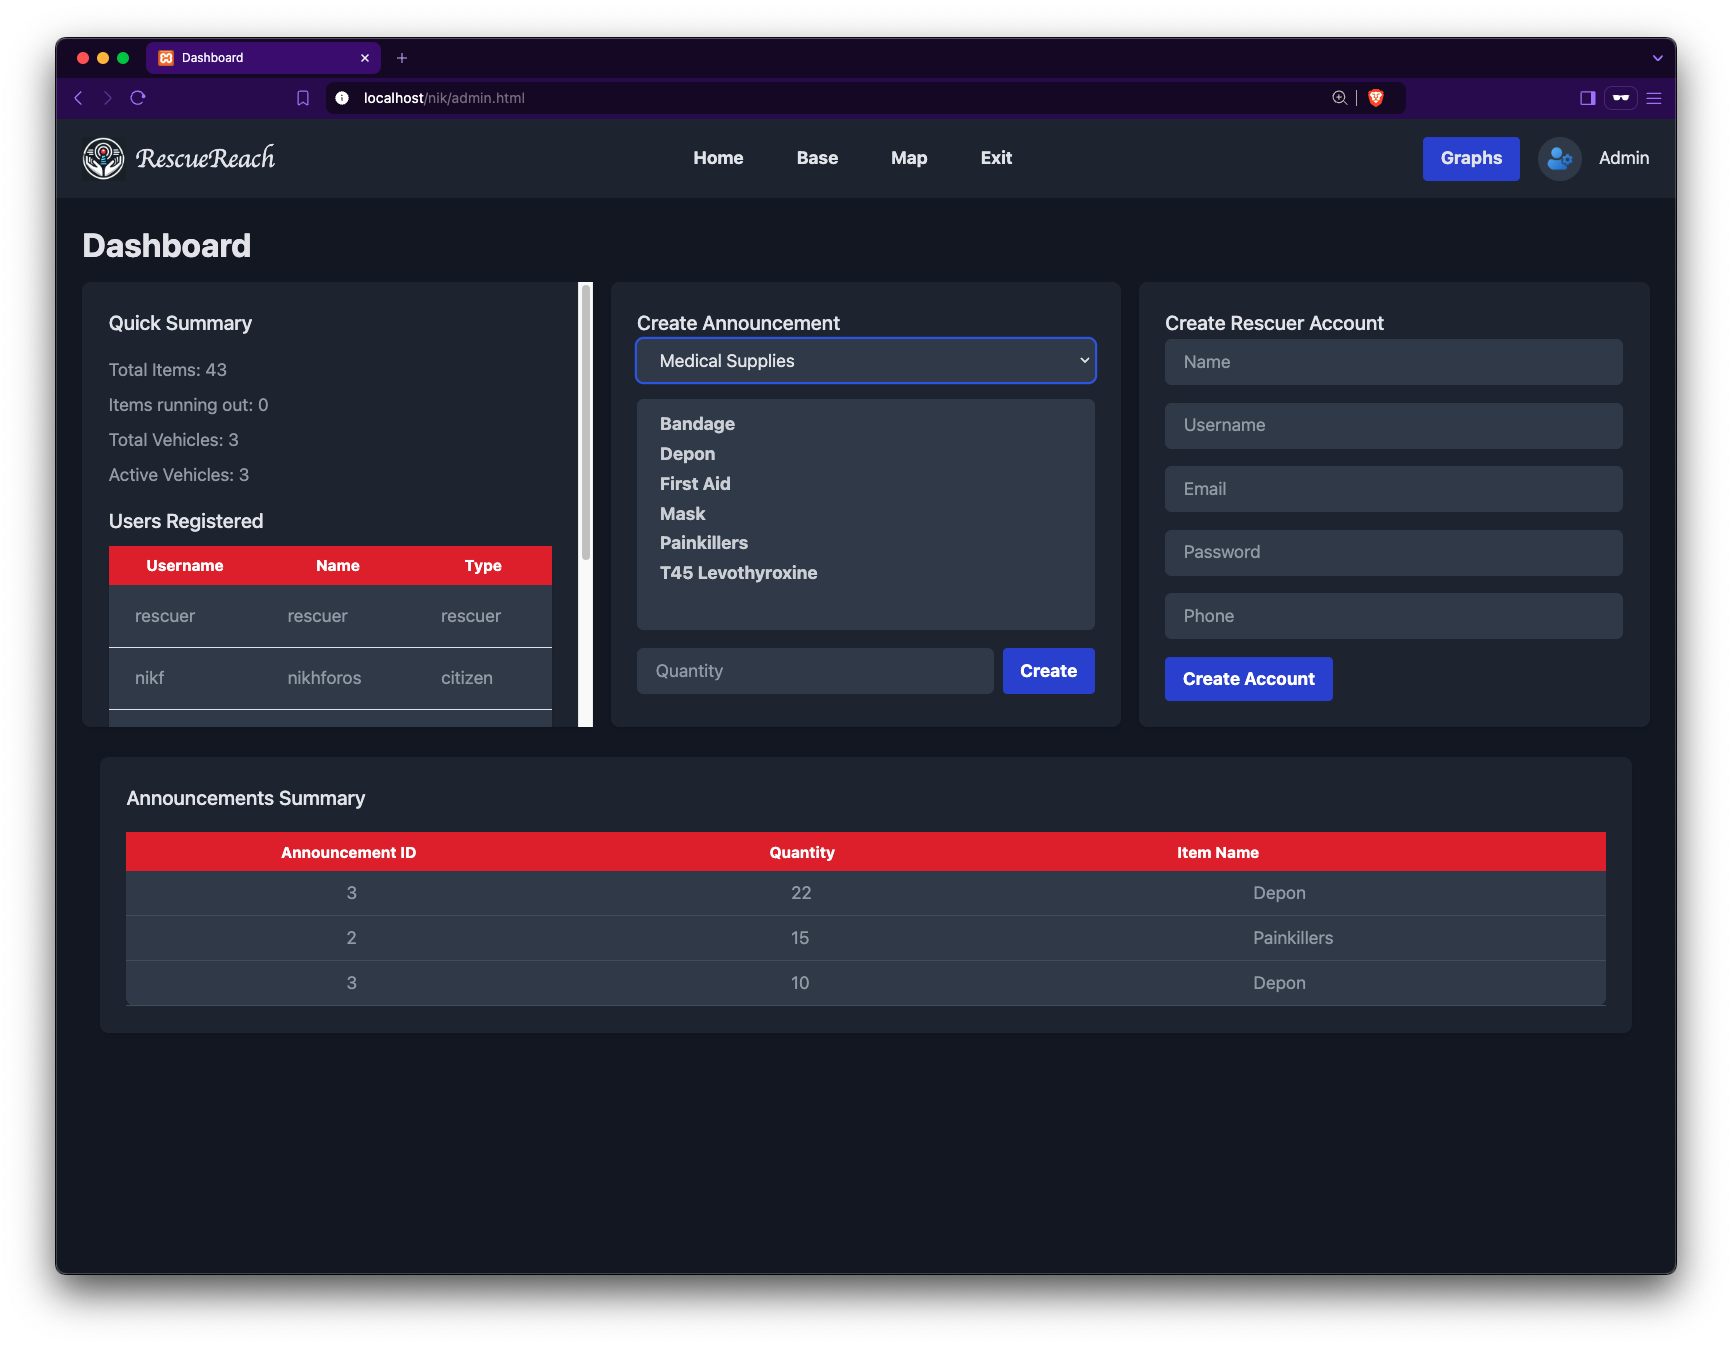
\includegraphics[width=0.9\textwidth]{img/admin-dashboard}
        \vspace{-1em}
        \caption{Dashboard admin}
    \end{figure}

    Το αρχείο \c{dashboard.js} χειρίζεται τη συγκεκριμένη σελίδα.
    Στην αρχή καλούνται όλες οι απαραίτητες συναρτήσεις για την εμφάνιση των διαφόρων modules.

    \subsection{Quick Summary}
        Η συνάρτηση \c{loadDashboardSummary()} στέλνει ένα AJAX request στο \c{summary.php}, ζητώντας τον συνολικό αριθμό των items (\c{#totalItems}),
            και τον αριθμό των items που τελειώνουν (\c{#lowStockItems}), και επιστρέφονται σε JSON μορφή.
        Αντίστοιχα η \c{fetchActiveVehicles()} στέλνει ένα AJAX request στο \c{active\_vehicles.php}, ζητώντας τον αριθμό των vehicles που είναι ενεργά (\c{#activeVehicles}).
        Η \c{registeredUsers()} δέχεται δεδομένα από το \c{registered\_users.php}, και μέσω της \c{populateTable()} εμφανίζει έναν πίνακα με τους εγγεγραμμένους χρήστες.

    \subsection{Create Announcement}
        Για τη φόρτωση των διαφορετικών κατηγοριών των items για τη δημιουργία της ανακοίνωσης, καλείται αρχικά η \c{loadCategoriesAndItems()}
        η οποία στέλνει ένα AJAX request στο \c{announchment.php}.
        Η PHP επιστρέφει ένα JSON αρχείο της μορφής:

        \begin{graycomment}
            \verb|{"categories": [id, name], "items": [id, name, category_id]}|
        \end{graycomment}

        Τα δεδομένα που επιστρέφονται χρησιμοποιούνται από τη \c{loadDashboardSummary()} για να γίνουν populate οι κατηγορίες της φόρμας.
        Αν ο χρήστης επιλέξει μια κατηγορία, η \c{filterItemsByCategory()} κάνει populate τη λίστα με τα αντίστοιχα items μέσω του JSON αρχείου.

        Όταν πατηθεί το κουμπί \textbf{Create}, αποθηκεύονται σε μεταβλητές τα επιλεγμένα items, όπως επίσης και το πλήθος τους
        και στέλνονται στη \c{insert\_announchment.php}, η οποία τα κάνει insert στη βάση.
        Σε περίπτωση επιτυχίας στέλνεται το αντίστοιχο μήνυμα.

    \subsection{Create Rescuer Account}
        Όταν πατηθεί το κουμπί \textbf{Create Account}, καλείται η \c{createRescuerAccount()} η οποία μέσω Promise δημιουργεί μεταβλητές για κάθε value της φόρμας,
            τις οποίες στέλνει μέσω AJAX request στο \c{create\_rescuer.php}.
        Η PHP ελέγχει αν υπάρχει ήδη τέτοιο username ή email, στέλνει κατάλληλα echos αν υπάρχουν, και αν δεν υπάρχουν κάνει insert τον νέο χρήστη στη βάση δεδομένων.

    \subsection{Announcements Summary}
        Ακολουθείται παρόμοια διαδικασία με τη δημιουργία του πίνακα των εγγεγραμμένων χρηστών.
        Χρησιμοποιείται η \c{loadAnnouchmentSummary()} σε συνδυασμό με τη \c{get\_ann.php}.

    \subsection{Graphs}
        Το κουμπί \textbf{Graphs} ενεργοποιεί ένα modal\footnote{με κατάλληλη προσθαφαίρεση κλάσεων του Tailwind} με στατιστικά γραφήματα για τα requests και τα offers.

    \vspace{-1em}
    \begin{figure}[H] \noindent \centering
        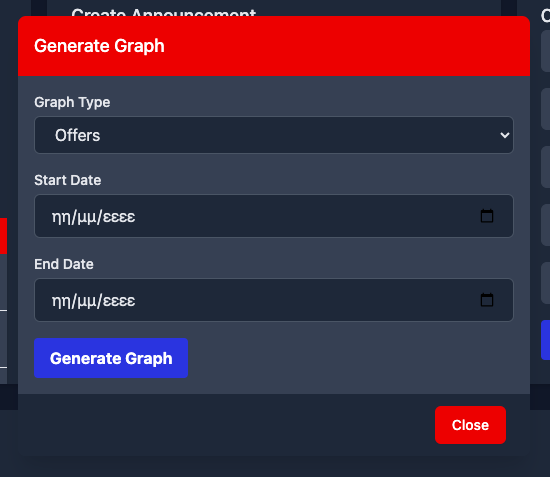
\includegraphics[width=0.9\textwidth]{img/admin-generate_graph}
        \vspace{-1em}
        \caption{Generate Graph model}
    \end{figure}
